% !TeX spellcheck = en_US
\documentclass[a4paper,12pt]{article}
\usepackage[utf8x]{inputenc}
\usepackage{wrapfig}
\usepackage{graphicx}
\usepackage{float}
\usepackage{listings}
\usepackage{amsmath}
\usepackage{caption}
\usepackage{subcaption}
\usepackage[usenames,dvipsnames,svgnames,table]{xcolor}

% Title Page
\title{AST2210 Report 2}
\author{Andreas Ellewsen}

\begin{document}
\maketitle
\tableofcontents
\section{Introduction}
This lab will go through basic use of CCD cameras, recording data, and how to analyze the images in IDL. 
\section{Image recording}
For the two first exercises the color Edmund Optics USB camera is used in a set-up with a white light lamp, a thin singlet lens, and a microscope objective. The program uc480viewer is used to control the camera. A picture is then taken of the white light source.

\subsection{Exercise 1}
There are many different settings to adjust in the program. This exercise focuses on three of them. These are 'histogram', 'value on horizon line', and 'camera properties'. 
Experimenting with the settings shows that 'Value on horizon line' brings up a graph of the intensity for red, green and blue, in the spot one chooses. 'Histogram' was forgotten when doing the lab. And 'Camera properties' brings up a window with three more settings. The first one is 'Pixel clock'. This changes the readout rate of the CCD. The second is 'Frame rate'. This changes the rate in which the program updates the picture. The last setting is 'Exposure time', which does exactly what one would expect. 

\subsection{Exercise 2}
The focus position of the microscope objective is then changed. It is observed that the color seen on the screen changes. Increasing the distance between the camera and the objective makes the picture more blue. Decreasing the distance makes it more red. Another thing to notice here is that, since we didn't manage to set everything in a perfectly straight line, the color of the dot (including the airy disk) didn't just change. It moved both vertically and horizontally. The maximum count for each color (with fixed exposure time) should have been checked, but this was overlooked during the lab. Nonetheless it was clear that they were not the same for any of them. Red was most intense, decreasing a little for each step closer to blue. The pictures can be seen in figure \ref{fig:Airy disks}.

\begin{figure}[H]
        \centering
        \begin{subfigure}[H]{0.5\textwidth}
                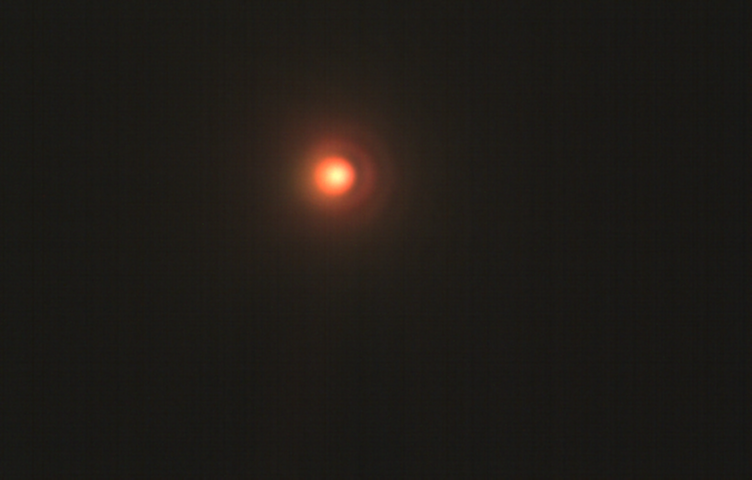
\includegraphics[width=\textwidth]{red}
                \caption{Red airy disk}
                \label{fig:red airy disk}
        \end{subfigure}%
        ~ %add desired spacing between images, e. g. ~, \quad, \qquad, \hfill etc.
          %(or a blank line to force the subfigure onto a new line)
        \begin{subfigure}[H]{0.5\textwidth}
                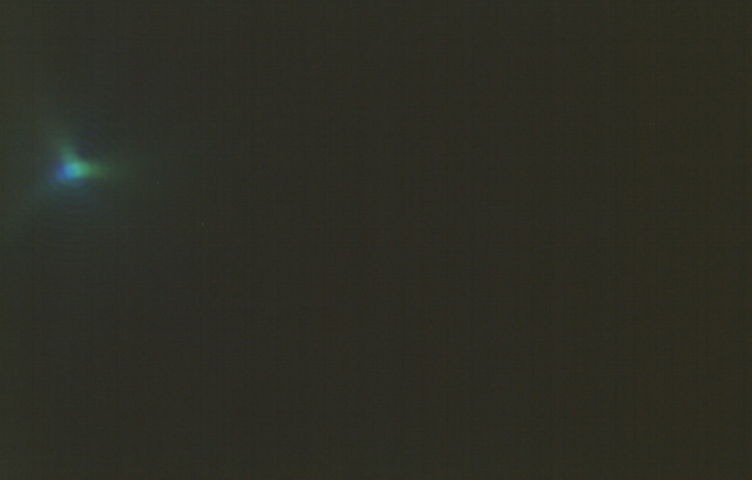
\includegraphics[width=\textwidth]{blue}
                \caption{Blue airy disk}
                \label{fig:blue airy disk}
        \end{subfigure}
        \caption{The pictures}\label{fig:Airy disks}
\end{figure}

\subsection{Exercise 3}
The camera is then changed to a monochromatic Edmund Optics USB Camera in a set-up with a laser and a 100 µm slit. 
Using the diffraction pattern on the live view of the camera, the width of the pixels in the sensor is measured (in µm). The uncertainty of the measurement is also calculated. 
This is done by using the formula for single-slit diffraction, $asin(\theta) = m\lambda$, where $a$ is the slit width, and $m$ the order of the minimum. Using basic trigonometry $sin(\theta)=p/D$, where D is distance between slit and camera, and p is distance from max to first minimum. During the lab, D was measured to be 15.8 $\pm$ 0.1 cm. This gives a distance between the two first minimums of $p= 1.090 \pm 0.007 mm$. Looking at the picture taken, the distance between the two minimums is $160 \pm 20 pixel$. Putting this together one gets a resolution of $6.926 \pm 0.909 µm/pixel$, which seems to be reasonable.

\subsection{Exercise 4}
A well exposed image of the diffraction pattern is recorded. Exposure time, frame rate and pixel clock of the image is noted. The image can been seen in figure \ref{fig:single slit}.The settings chosen for this image can be seen in table \ref{tab:Settings for image}.\\
\begin{table}[H]
\centering
\begin{tabular}{|l|l|}
\hline
Exposure time & 0.384 ms\\
Frame rate & 2.82 fps\\
Pixel clock & 40\\
\hline
\end{tabular}
\caption{Settings for image}\label{tab:Settings for image}
\end{table}

\begin{figure}[H]
\centering
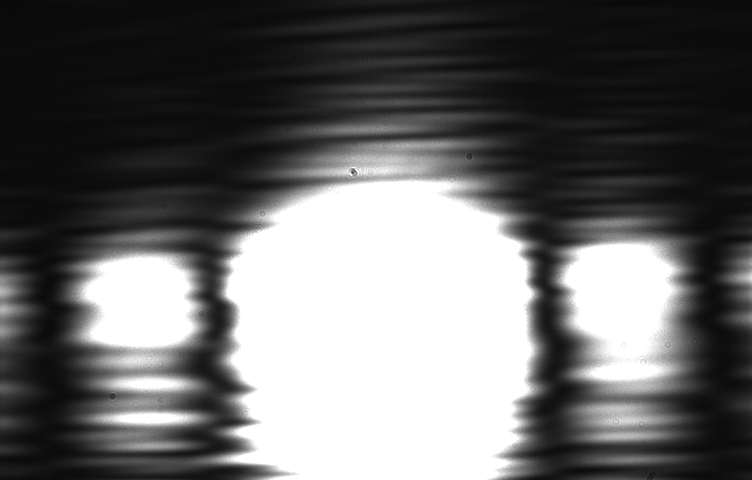
\includegraphics[width=\textwidth]{CCD_single_slit}
\caption{Single slit diffraction pattern}\label{fig:single slit}
\end{figure}

\subsection{Exercise 5}
The laser is then switched off, and the dust cover is put on the camera. The slit is then removed. A series of frames are then taken.
First we record 2 bias frames by turning down the exposure time to the minimum
value. Then we record 5 dark frames with the same exposure time as in exercise 4. And finally a dark frame at the maximum exposure time.
The dust cover of the camera is removed and a very basic type of flat field image is recorded by using a white paper to reflect light from the ceiling into the camera.
The integration time is adjusted so that the average pixel value is between halfway and one third of the maximum of the camera. This is done 16 times, noting the exposure time.
The dust cover is then put back on and 5 dark frames are recorded with the same exposure time.
The time that was used in this lab was 33.107 ms.
The pictures don't look very interesting, but some of them can been seen in figure \ref{fig:examples}.

\begin{figure}[H]
        \centering
        \begin{subfigure}[H]{0.3\textwidth}
                
\includegraphics[width=\textwidth]{bias1}
                \caption{Bias}
                \label{fig:bias}
        \end{subfigure}%
        ~ %add desired spacing between images, e. g. ~, \quad, \qquad, \hfill etc.
          %(or a blank line to force the subfigure onto a new line)
        \begin{subfigure}[H]{0.3\textwidth}
                
\includegraphics[width=\textwidth]{dark1}
                \caption{Dark current}
                \label{fig:dark current}
        \end{subfigure}
        ~ %add desired spacing between images, e. g. ~, \quad, \qquad, \hfill etc.
          %(or a blank line to force the subfigure onto a new line)
        \begin{subfigure}[H]{0.3\textwidth}
                
\includegraphics[width=\textwidth]{flat1}
                \caption{Flatfield}
                \label{fig:flatfield}
        \end{subfigure}
        \caption{Examples of pictures taken}\label{fig:examples}
\end{figure}

\section{Post processing}

\subsection{Exercise 6}
We start by loading one bias frame, and the dark frame with maximum exposure time into IDL. Average,minimum, and maximum pixel values are computed for both and can be seen in table \ref{tab:values for image}. The histograms of the pixel values is plotted in figure \ref{fig:histograms}.\\
\begin{table}[H]
\begin{center}
\begin{tabular}{|l|l|l|}
\hline
 & Bias1 & Darkmax \\
\hline
Average & 9.38291 & 11.0843\\
Minimum & 7 & 8\\
Maximum & 16 & 94\\
\hline
\end{tabular}
\caption{Average, max, and min for the two pictures}
\label{tab:values for image}
\end{center}
\end{table}

\begin{figure}[H]
        \centering
        \begin{subfigure}[H]{0.5\textwidth}
                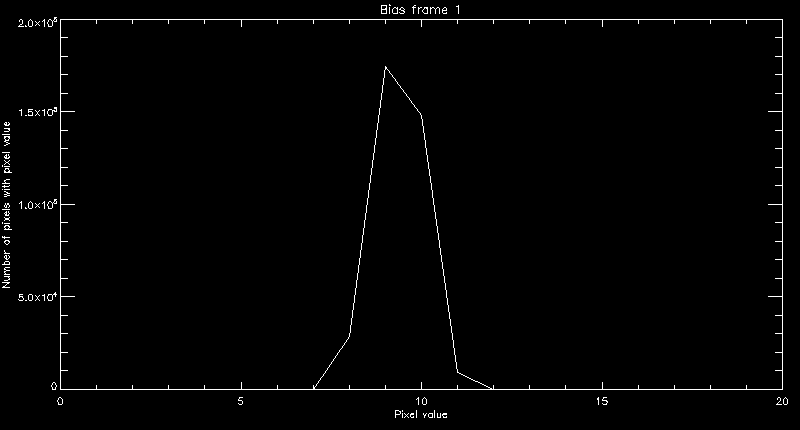
\includegraphics[width=\textwidth]{histogram1.png}
                \caption{Histogram of Bias 1}
                \label{fig:histbias1}
        \end{subfigure}%
        ~ %add desired spacing between images, e. g. ~, \quad, \qquad, \hfill etc.
          %(or a blank line to force the subfigure onto a new line)
        \begin{subfigure}[H]{0.5\textwidth}
                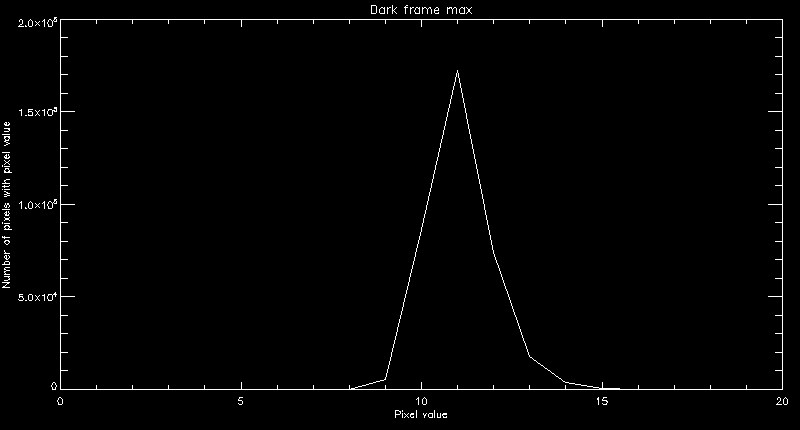
\includegraphics[width=\textwidth]{histogram2.png}
                \caption{Histogram of Bias 2}
                \label{fig:histbias2}
        \end{subfigure}
        \caption{The histograms for each of the bias frames}\label{fig:histograms}
\end{figure}

Examining the frames one notices that there are some differences between the two frames. The biggest difference is that the mean pixel value is different for the two. When locating the pixels with the maximum value for both images it is found that they are not the same. This is not as expected, since one would assume that the "sensitive" pixel should be the same pixel for both frames.

All of this is done using the IDL code below:  
\lstinputlisting[language=IDL,frame=L,lastline=30]{ex6.pro}

\subsection{Exercise 7}
Next we load both bias frames, add them together, and measure the mean value of the central square region, 300pixels on a side. The quantity referred to as the mean value here is $\overline{B_1} + \overline{B_2}$. Subtracting one bias frame from the other, and measuring the standard deviation for the central region gives $\sigma_{B_1-B_2}$
All of this is done using the IDL code below: 
\lstinputlisting[language=IDL, frame=L, firstline=5, lastline=15]{ex7.pro}
\subsection{Exercise 8}
Any fixed bias patterns are then removed by subtracting the two bias frames, leaving just the noise from the two bias frames $\sigma_{B_1-B_2}$. This should be $\sqrt{2}$ times the noise of one bias frame. This is used later, when calculating the noise in the flat fields as we increase the number of flat fields we use.
\subsection{Exercise 9}
The same is done for two flat frames, giving us $\overline{F_1} + \overline{F_2}$, and $\sigma_{F_1-F_2}$. All of this is done using the IDL code below: 
\lstinputlisting[language=IDL, frame=L, firstline=18, lastline=28]{ex7.pro}
\subsection{Exercise 10}
The measurements done so far have been done in pixel counts, or analog-to-digital units (ADU). There is a conversion factor $g$ that relates 1 ADU to the number of actually measured electrons. And since one can expect the signal to display Poisson statistics measured in electrons, one expects $\sigma_electrons = \sqrt{F_{electrons}}$. In this case both $\sigma$ and $F$ have been multiplied by this factor, and thus we have $g\sigma_{electrons} = \sqrt{gF_{electrons}}$.
Solving for g:
\begin{equation}
g = \frac{F_{electrons}}{\sigma_{electrons}^2} [electrons/ADU].
\end{equation}
Correcting for bias and noise related to bias:
\begin{equation}
g = \frac{(\overline{F_1}+\overline{F_2})-(\overline{B_1}+\overline{B_2})} {(\sigma_{F_1-F_2}^2)-(\sigma_{B_1-B_2}^2)} [electrons/ADU]
\end{equation}
With all the information gathered so far one can compute this conversion factor $g$. Thus one finds that in this case: $ g = 0.0107027 [electrons/ADU]$
This is done using the IDL code below: 
\lstinputlisting[language=IDL, frame=L, firstline=31, lastline=32]{ex7.pro}

\subsection{Exercise 11}
The only source of noise in a bias frame should be the readout noise. 
This noise is calculated in the following program, and is found to be 1.07906 electrons per pixel.
\lstinputlisting[language=IDL, frame=L, firstline=35, lastline=36]{ex7.pro}

\subsection{Exercise 12}
By adding the flats together and plotting the noise one can see that the noise is reduced by adding more flats. Unfortunately one of the flat fields taken in the lab was corrupt. Because of this I chose to use only 14 flats. The resulting plot can be seen in figure \ref{fig:noise in flats}.

\begin{figure}[H]
\centering
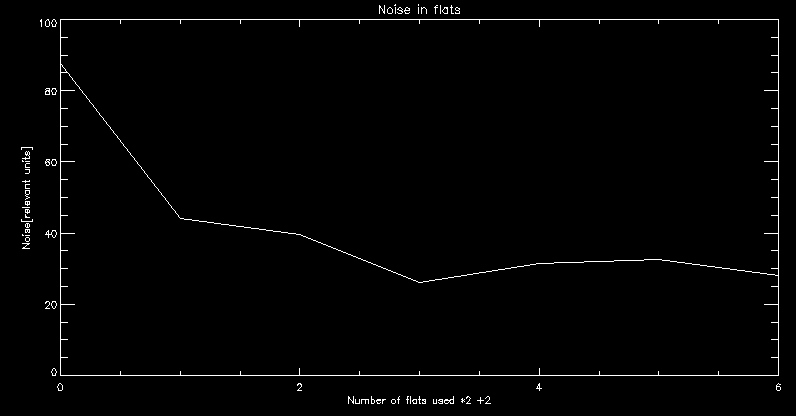
\includegraphics[width=\textwidth]{Noiseinflats}
\caption{Noise reduction in flats}\label{fig:noise in flats}
\end{figure}
This was generated by the following code:
\lstinputlisting[language=IDL, frame=L, firstline=39, lastline=84]{ex7.pro}
	
\subsection{Exercise 13}
Finally, all of the frames will be used to correct the diffraction image. This is done using the following formula:
\begin{equation}
\frac{Raw image-Dark_R}{Flat-Dark_F}\times m = Corrected image
\end{equation}
Where $Dark_R$ is a 'master dark frame'. This 'master dark frame' is the basically the picture you get if you take the average of all the dark frames with the same exposure time as the raw image and make one picture out of it. $Dark_F$ is the "master dark frame" made in the exact same way, only using the darks with the same exposure time as the flats. And $m = avg(F-Dark_F)$.
This was generated by the following code:
\lstinputlisting[language=IDL, frame=L,firstline=91, lastline=114]{ex7.pro}
\section{Conclusion}
The result of this is a corrected image, which can be seen in figure \ref{fig:Raw image} along with the raw image in figure \ref{fig:Corrected}. One must admit that there is little improvement to be seen. This is probably because of the way the flat fields were made. The illumination was obviously not uniform which it ideally should have been.
\begin{figure}[H]
\centering
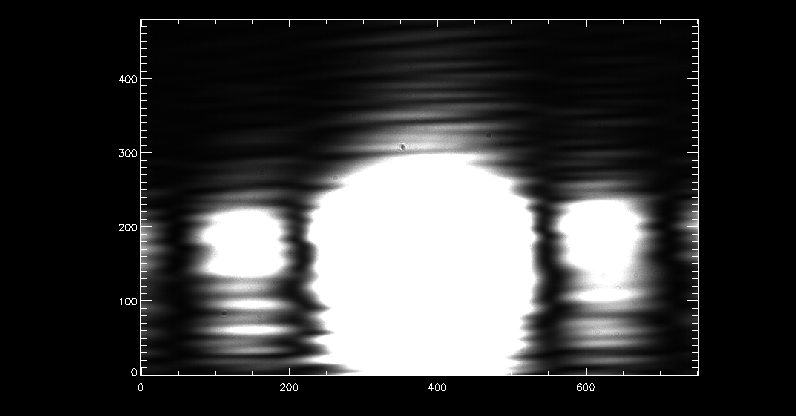
\includegraphics[width=\textwidth]{Raw_image}
\caption{Raw image}\label{fig:Raw image}
\end{figure}
\begin{figure}[H]
\centering
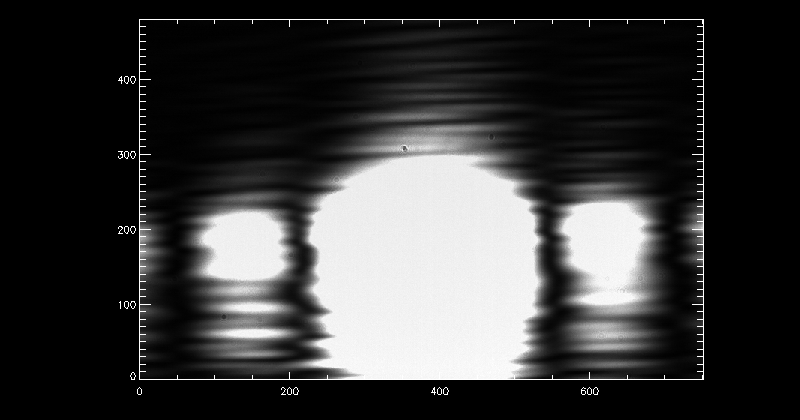
\includegraphics[width=\textwidth]{Corrected}
\caption{Corrected image}\label{fig:Corrected}
\end{figure}
\end{document}
